% Version 3.1 December 2024
% See section 11 of the User Manual for version history
%
%%%%%%%%%%%%%%%%%%%%%%%%%%%%%%%%%%%%%%%%%%%%%%%%%%%%%%%%%%%%%%%%%%%%%%
%%                                                                 %%
%% Please do not use \input{...} to include other tex files.       %%
%% Submit your LaTeX manuscript as one .tex document.              %%
%%                                                                 %%
%% All additional figures and files should be attached             %%
%% separately and not embedded in the \TeX\ document itself.       %%
%%                                                                 %%
%%%%%%%%%%%%%%%%%%%%%%%%%%%%%%%%%%%%%%%%%%%%%%%%%%%%%%%%%%%%%%%%%%%%%

% ============================================================================
% EDIT LOG (for author review before submission)
%
% Everything marked "% [AI-EDITED ...]" below was written or rewritten by an
% AI assistant on 2026-07-17, grounded in the verified implementation
% (env/weekly_retail_env.py, agent/q_learning.py, agent/sarsa.py,
% agent/sac_alphalr.py, dashboard/backend/rollout.py) and in paper_v1.md.
% Please review each marked block before submission.
%
% Key structural change from the previous draft: the Introduction and
% Literature Review previously described a TWO-ECHELON (warehouse + retail)
% system optimized with PPO. The code that actually runs
% (env/weekly_retail_env.py) is SINGLE-ECHELON (retail floor only, no
% intermediate warehouse, zero lead time) and compares FOUR policies
% (Random, Q-learning, SARSA, SAC with adaptive temperature -- no PPO). Per
% author instruction, the Introduction, Literature Review, and comparison
% table were rewritten to match the single-echelon, four-policy system so
% the whole paper is internally consistent with the running code.
%
% Sections removed entirely (Springer template boilerplate/demo content,
% not applicable to this paper): the demo "Equations", "Tables", "Figures",
% "Algorithms/Program codes and Listings" (verbatim Pascal/exponentiation
% examples), "Cross referencing", and "Theorem-like environments" sections,
% plus their unused preamble packages/environments (listings, unused
% amsthm theorem styles). A single real \begin{algorithm} block for the
% Q-learning/SARSA update rule was kept/rewritten with real content.
% ============================================================================

\documentclass[pdflatex,sn-mathphys-num]{sn-jnl}% Math and Physical Sciences Numbered Reference Style

%%%% Standard Packages
\usepackage{graphicx}%
\usepackage{multirow}%
\usepackage{amsmath,amssymb,amsfonts}%
\usepackage[title]{appendix}%
\usepackage{xcolor}%
\usepackage{textcomp}%
\usepackage{manyfoot}%
\usepackage{booktabs}%
\usepackage{algorithm}%
\usepackage{algorithmicx}%
\usepackage{algpseudocode}%
%%%%

% [AI-EDITED 2026-07-17] The sn-jnl class ships with a narrow "smallcond"
% text block (131mm wide on an A4 page) and a large reserved footskip,
% which leaves wide empty side margins and a big gap below the text before
% the footer. Overriding geometry here switches to standard A4 print
% margins with a normal-width text block.
\usepackage{geometry}%
\geometry{
    a4paper,
    top=25mm,
    bottom=25mm,
    left=25mm,
    right=25mm,
    headheight=14pt,
    headsep=10mm,
    footskip=15mm
}%

\raggedbottom

\begin{document}

\title[RL for Weekly Retail Inventory Replenishment]{Reinforcement Learning for Weekly Retail Inventory Replenishment: A Comparison of Tabular and Deep Actor-Critic Methods}
% [AI-EDITED] Title updated to match the single-echelon, four-policy study
% actually implemented and evaluated (was "Reinforcement Learning with
% Inventory Inbounding"). Please confirm this is the title you want to
% submit under.

\author*[1]{\fnm{Hao Trieu Quoc} \sur{Author}}\email{haotqse180011@fpt.edu.vn}

\author[1]{\fnm{Duy Nguyen Van Anh} \sur{Author}}\email{duynvase181823@fpt.edu.vn}
\equalcont{These authors contributed equally to this work.}

\author[1]{\fnm{Thu Nguyen Thi Minh} \sur{Author}}\email{thuntmse185043@fpt.edu.vn}
\equalcont{These authors contributed equally to this work.}

\affil*[1]{\orgdiv{Department of Artificial Intelligence}, \orgname{FPT University}, \orgaddress{\street{7 D1 Street, Tang Nhon Phu}, \city{Ho Chi Minh City}, \postcode{700000}, \country{Vietnam}}}

% [AI-EDITED] Abstract rewritten from placeholder text to match paper_v1.md.
\abstract{Retail inventory replenishment is a sequential decision problem in which a store manager must decide, week by week, how many units of each product to order from a distributor while balancing revenue, procurement cost, storage cost, and stockout cost under a hard physical constraint on retail floor space. This paper formulates the problem as a Markov Decision Process (MDP) for a five-category Apple retail store (iPhone, iPad, MacBook, Apple Watch, AirPods) and compares four ordering policies: a uniform random baseline, tabular Q-learning, tabular SARSA, and a Soft Actor-Critic variant with adaptive entropy temperature, denoted SAC-AlphaLR. The revised environment uses net profit, rather than negative cost alone, as the learning signal and applies a common 40\% retail markup. All policies are evaluated over a simulated 52-week horizon with seasonal and holiday-aware stochastic demand. SAC-AlphaLR achieves the lowest annual cost (156.78 billion VND), the highest revenue (181.55 billion VND), the highest net profit (24.77 billion VND), and the fewest stockout units (2{,}039). Q-learning and SARSA also become profitable, earning 16.06 and 8.84 billion VND respectively, whereas the random policy remains unprofitable.}

\keywords{Reinforcement Learning, Inventory Management, Retail Replenishment, Soft Actor-Critic, Q-learning, SARSA, Markov Decision Process}
% [AI-EDITED] Keywords filled in (was "keyword1, Keyword2, Keyword3, Keyword4").

\maketitle

\section{Introduction}\label{sec1}
% [AI-EDITED] Rewritten to describe the single-echelon, floor-space-constrained
% retail system with four compared policies, replacing the previous
% two-echelon / PPO framing.

Inventory management is a fundamental challenge in retail operations, requiring firms to balance product availability against operational cost efficiency. Excess inventory increases holding costs and ties up working capital, whereas insufficient inventory results in stockouts, lost sales, and reduced customer satisfaction. Classical inventory control methods, including the Economic Order Quantity (EOQ) model~\cite{bib6}, the newsvendor model~\cite{bib7}, and $(s,S)$ policies~\cite{bib8}, have long been used to address this trade-off, and Clark and Scarf~\cite{bib4} extended these ideas to coordinated multi-echelon control through echelon base-stock policies. These classical approaches generally rely on stationary demand assumptions and fixed decision rules, which limits their effectiveness in environments with seasonal fluctuations, promotional events, and a hard physical constraint on how much stock a store can actually hold.

Reinforcement Learning (RL) offers a data-driven alternative for sequential decision-making, letting an agent learn a replenishment policy through interaction with a simulated environment rather than relying on a predefined mathematical model~\cite{bib2}. In a commercial replenishment setting, the learning objective must credit revenue as well as charge operating costs; otherwise an agent can reduce its objective by ordering too little even when that behavior destroys sales. Tabular methods such as Q-learning~\cite{bib20} and SARSA~\cite{bib21} learn action-value estimates directly over a discretized state space and remain attractive for their simplicity and interpretability. Deep Reinforcement Learning (DRL) extends this idea with function approximation: among modern DRL algorithms, Soft Actor-Critic (SAC)~\cite{bib3} and its adaptive-temperature variant~\cite{bib23} have demonstrated strong performance in continuous control problems by maximizing a trade-off between expected return and policy entropy, which makes SAC well suited to a continuous order-quantity action space.

Recent studies have shown the potential of DRL for inventory optimization across lost-sales, dual-sourcing, and multi-echelon settings~\cite{bib5}. Zhang, He, and Zheng~\cite{bib1} proposed a DRL-based dynamic replenishment framework for a multi-echelon FMCG (fast-moving consumer goods) supply chain, formulating replenishment as an MDP and using an improved SAC variant, adopted in this paper as the SAC-AlphaLR policy (Section~\ref{subsec:sac}), to coordinate a manufacturer-warehouse-retailer chain, with reported cost improvements over overstocking, particle swarm optimization, and standard SAC baselines. Comparable studies~\cite{bib16,bib17,bib18,bib19} similarly target multi-echelon coordination, generally under a single product and a stationary or synthetic demand process.

Despite this progress, two gaps remain relevant to specialty electronics retail. First, most existing DRL inventory studies assume either a single product or a stationary demand process, which does not reflect the pronounced day-of-week, seasonal, and holiday-driven demand swings observed in consumer electronics retail. Second, and more specifically, prior work on constrained inventory systems typically models capacity as an echelon-level warehouse limit rather than as a single, shared retail floor-space budget (measured in square meters) across several product categories with different per-unit footprints; this latter constraint does not decompose into independent per-product problems, since ordering more of one product directly reduces the floor budget available to the others. Third, few studies benchmark a spectrum of RL algorithms, from simple tabular methods to deep actor-critic methods, on the same environment and evaluation protocol, which makes it difficult to judge how much of a deep method's advantage is attributable to the algorithm itself versus differences in experimental setup.

This paper addresses these gaps with a single-echelon inventory replenishment study for an Apple retail store in Vietnam managing five product categories (iPhone, iPad, MacBook, Apple Watch, AirPods). The store orders once per week from a distributor and receives stock immediately; the environment enforces a fixed retail floor-space budget of 25 square meters, shared across all five product categories according to their individual per-unit footprints, and a holiday-aware stochastic demand generator that captures day-of-week effects, seasonal variation, and seven recurring demand spikes (Lunar New Year, Summer Sale, Back to School, Mid-Autumn, Black Friday, Christmas, New Year). Replenishment is formulated as an MDP, and four ordering policies, a random baseline, tabular Q-learning, tabular SARSA, and a Soft Actor-Critic agent with adaptive temperature (SAC-AlphaLR), are trained and evaluated under an identical protocol.

The main contributions of this work are summarized as follows:

\begin{itemize}
    \item A single-echelon retail inventory simulation environment constrained by a shared retail floor-space budget (in square meters) across five product categories with distinct per-unit footprints and cost structures.

    \item A holiday-aware stochastic demand generation model that captures day-of-week effects, seasonal variation, and seven recurring promotional/holiday events characteristic of consumer electronics retail.

    \item An MDP formulation of weekly retail replenishment under this shared floor-space constraint, with a 26-dimensional state and a 5-dimensional order-quantity action.

    \item A controlled empirical comparison of four ordering policies, a random baseline, tabular Q-learning, tabular SARSA, and Soft Actor-Critic with adaptive temperature, trained and evaluated under an identical protocol on the same environment.

    \item Transparent verification of all reported hyperparameters, cost structures, and results against the running implementation, with explicit documentation of the points where an earlier design draft of this project diverged from the final, tuned system.
\end{itemize}

The remainder of this paper is organized as follows. Section~\ref{sec2} reviews related work in classical and RL-based inventory management. Section~\ref{sec3} presents the proposed methodology, including the environment, demand model, and the four ordering policies. Section~\ref{sec4} describes the experimental setup. Section~\ref{sec5} reports the results. Section~\ref{sec6} discusses the findings. Section~\ref{sec7} discusses limitations and future work. Section~\ref{sec8} concludes the paper.

\section{Literature Review}\label{sec2}

\subsection{Classical Inventory Management}

Inventory management has long been a cornerstone of operations research, with foundational models establishing the theoretical basis for replenishment decisions under uncertainty. The Economic Order Quantity (EOQ) model, introduced by Harris~\cite{bib6}, provided a closed-form solution for balancing ordering and holding costs under deterministic, stationary demand. While elegant in its simplicity, the EOQ model's reliance on constant demand and instantaneous replenishment rendered it unsuitable for stochastic environments. The newsvendor model~\cite{bib7} extended inventory theory to single-period perishable products under demand uncertainty, offering a trade-off between overstocking and understocking costs. However, its single-period structure inherently limits applicability to multi-period, continuous-review settings.

The $(s,S)$ policy, formally proven optimal by Scarf~\cite{bib8} for periodic-review inventory systems with fixed ordering costs, addressed multi-period dynamics by establishing threshold-based replenishment: an order is placed when inventory falls below $s$, raising it to $S$. Similarly, base-stock policies emerged as optimal for systems without fixed costs, where the optimal decision is to order up to a target level each period. Clark and Scarf~\cite{bib4} generalized these concepts to multi-echelon structures, demonstrating that echelon-based inventory policies could achieve near-optimal performance in serial supply chains. Dynamic programming (DP), formalized by Bellman~\cite{bib9}, provided a rigorous mathematical framework for sequential decision-making under uncertainty and became the standard approach for solving stochastic inventory problems.

Despite their theoretical elegance, these classical methods share fundamental limitations. They assume demand follows a known stationary distribution, which rarely holds in practice, particularly in consumer electronics retail where demand exhibits seasonality, holiday spikes, and day-of-week patterns. They rely on fixed policy parameters that cannot adapt to changing market conditions. Furthermore, DP suffers from the curse of dimensionality: as the number of products and state variables grows, exact solutions become computationally intractable. None of these classical formulations natively handles a single shared capacity constraint (such as retail floor space, expressed in square meters) across several products with different physical footprints, since doing so couples what would otherwise be independent single-product inventory problems. These limitations motivate data-driven, adaptive approaches capable of learning inventory policies directly from experience.

\subsection{Reinforcement Learning for Inventory Management}

Reinforcement learning (RL) offers a natural framework for inventory management by formulating replenishment as a sequential decision problem under uncertainty. The inventory manager (agent) observes the current state (inventory levels, demand forecast, and economic attributes), takes an action (order quantities), and receives a reward equal to scaled operating profit: sales revenue less procurement, holding, and shortage expenses. This MDP formulation captures the dynamics, uncertainty, and long-term economic implications inherent in inventory control.

Tabular RL methods learn action-value estimates over a discretized state space without function approximation. Q-learning~\cite{bib20} is an off-policy temporal-difference method that bootstraps toward the maximum action-value of the next state, while SARSA~\cite{bib21} is its on-policy counterpart, bootstrapping toward the value of the action actually selected next under the current exploration policy; Sutton and Barto~\cite{bib22} provide the standard treatment of both, including their convergence properties and the exploration-exploitation trade-off. Deep Reinforcement Learning (DRL) extends RL with neural function approximation, enabling tractable solutions in high-dimensional state and action spaces. Deep Q-Networks (DQN)~\cite{bib10} approximate the Q-function with a neural network and have demonstrated success in discrete action spaces, but are inherently limited to discrete actions. Deep Deterministic Policy Gradient (DDPG)~\cite{bib11} addressed this with an actor-critic architecture for continuous action spaces. Proximal Policy Optimization (PPO)~\cite{bib12} introduced clipped surrogate objectives for stable on-policy updates. Soft Actor-Critic (SAC)~\cite{bib3} further improved sample efficiency and exploration by maximizing entropy alongside expected return, and a follow-up formulation~\cite{bib23} replaced its fixed entropy-temperature hyperparameter with an automatically tuned value, which is the formulation adopted in this paper (Section~\ref{subsec:sac}).

In the inventory domain, DRL has shown considerable promise. Oroojlooyjadid et al.~\cite{bib13} applied DQN to the multi-period newsvendor problem and demonstrated that RL-based policies could outperform traditional optimization approaches by learning from demand realizations. Gijsbrechts et al.~\cite{bib5} conducted a comprehensive evaluation of DRL across lost-sales, dual-sourcing, and multi-echelon inventory problems, finding that DRL policies could match or exceed optimized base-stock policies, particularly in settings where closed-form solutions are unavailable, for example under lost-sales dynamics or capacity constraints that break the assumptions behind classical heuristics. Kegenbekov and Jackson~\cite{bib14} developed an adaptive supply chain framework using DRL and showed that learned policies could synchronize demand and supply under non-stationary conditions. Tian et al.~\cite{bib15} proposed an improved actor-critic architecture with PPO for warehouse inventory replenishment, demonstrating cost reductions relative to rule-based policies.

These studies collectively demonstrate that DRL can discover effective inventory policies without explicit assumptions about demand distributions. However, most simplify demand generation to stationary or weakly non-stationary processes, and few directly compare a spectrum of RL algorithms of differing complexity, from tabular to deep actor-critic, under an identical environment and evaluation protocol; this comparison is one of the goals of the present study.

\subsection{Deep Reinforcement Learning for Multi-Echelon and Constrained Inventory Systems}

A separate line of DRL inventory research targets multi-echelon coordination, where the complex interaction between echelons, upstream ordering decisions affecting downstream availability and vice versa, demands policies that account for system-wide dynamics. Zhang, He, and Zheng~\cite{bib1} proposed a DRL-based dynamic replenishment approach (ME-DRFO) for a multi-echelon FMCG inventory system comprising a manufacturer, a warehouse, and a retailer, modeling the problem as an MDP and using an improved Soft Actor-Critic variant termed SAC-AlphaLR to learn replenishment policies. Their study reported a 12.31\% replenishment-cost reduction and a reduction in inventory shortages to 2.21\%, relative to overstocking, particle swarm optimization, and standard SAC baselines, but modeled a single product under stationary normal demand and did not represent a shared physical capacity constraint across products. The present implementation retains the SAC-AlphaLR name to identify the deep actor-critic policy derived from this research direction. Kaynov et al.~\cite{bib16} studied a one-warehouse multi-retailer system with policy-gradient DRL under correlated demand across retailers but retained stationary demand and no capacity constraints. Hammler et al.~\cite{bib17} developed fully dynamic reorder policies for multi-echelon systems that adapted to demand pattern changes through retraining, though demand generation remained synthetic. Cheng et al.~\cite{bib18} proposed a radial basis function DQN for a three-echelon setting with a single product under stationary demand. Lu et al.~\cite{bib19} extended multi-echelon DRL to supply disruption scenarios without retail-specific temporal demand patterns.

Gijsbrechts et al.~\cite{bib5}, evaluating DRL across several problem classes including a multi-echelon serial system, found that DRL performance degraded as system complexity increased, and that DRL offered the largest advantage over classical heuristics precisely when the problem's constraint structure departed from the assumptions under which those heuristics are provably optimal. The environment studied in this paper departs from the classical single-product setting in an analogous but distinct way: rather than coordinating ordering decisions across supply-chain echelons, it couples five product categories through a single shared retail floor-space budget, so that an agent cannot solve each product's inventory problem independently. This constraint structure, and the systematic comparison of tabular against deep actor-critic methods under it, is not addressed by the multi-echelon studies reviewed above.

\begin{table*}[t]
\centering
\caption{Comparison of DRL-Based Inventory Studies}
\label{tab:comparison}
\renewcommand{\arraystretch}{1.2}
\resizebox{\textwidth}{!}{%
\small
\begin{tabular}{p{2.2cm}p{1.8cm}p{2.2cm}p{2.0cm}p{1.8cm}p{2.6cm}p{2.8cm}}
\hline
\textbf{Study} &
\textbf{Supply Chain} &
\textbf{Inventory Structure} &
\textbf{DRL Algorithm(s)} &
\textbf{Demand Model} &
\textbf{Operational Constraints} &
\textbf{Main Limitations} \\
\hline
Zhang et al.~\cite{bib1} & Multi-echelon (M-W-R) & Single product & SAC-AlphaLR (improved SAC) & Stationary normal & None & Single product; stationary demand; no capacity constraints \\
Kaynov et al.~\cite{bib16} & 2-echelon (W-MR) & Single product, multiple retailers & Policy gradient & Stationary normal & None & Stationary demand; no capacity constraints; retail-specific patterns absent \\
Hammler et al.~\cite{bib17} & Multi-echelon & Single product & DQN, PPO & Synthetic pattern & None & Synthetic demand; no holiday effects; single product \\
Cheng et al.~\cite{bib18} & 3-echelon & Single product & RBF-DQN & Stationary normal & Lead time & Single product; stationary demand; limited operational constraints \\
Gijsbrechts et al.~\cite{bib5} & Serial, divergent & Single product & DQN, PPO & Stationary & Lead time & Performance degrades with complexity; no retail demand patterns \\
Lu et al.~\cite{bib19} & Multi-echelon & Single product & DQN & Disruption scenarios & Disruption events & Single product; disruption-focused; no consumer electronics retail \\
\textbf{This Work} & 1-echelon (Retail only) & 5 product categories & Random, Q-learning, SARSA, SAC (adaptive temperature) & Day-of-week, seasonal, holiday, stochastic & Shared retail floor-space budget (m\textsuperscript{2}), per-product footprint, per-product order cap & Single fixed evaluation run; no lead time, upstream warehouse echelon, or confidence intervals \\
\hline
\end{tabular}%
}
\end{table*}
% [AI-EDITED] "This Work" row rewritten to match the single-echelon, four-policy,
% floor-space-constrained system in env/weekly_retail_env.py. The other rows
% (prior studies) are unchanged from the original draft.

\subsection{Research Gap Summary}
% [AI-EDITED] Rewritten to match the single-echelon, floor-space-constrained,
% algorithm-comparison framing.

The preceding review reveals two persistent gaps relevant to this study. First, classical inventory models assume stationary demand and fixed policy parameters, while existing DRL studies, despite demonstrating adaptability, are typically evaluated under stationary or weakly non-stationary synthetic demand that does not reflect the day-of-week seasonality, holiday surges, and stochastic variation characteristic of consumer electronics retail. Second, the DRL inventory literature has concentrated on multi-echelon coordination under single-product, uncapacitated (or lead-time-only) settings; the complementary problem of several product categories sharing one physical capacity constraint at a single echelon, and the resulting need to trade off products against one another for the same floor space, has not been directly addressed. Nor has prior work systematically compared tabular RL methods (Q-learning, SARSA) against a deep actor-critic method (SAC) on the same environment and evaluation protocol to isolate the contribution of model capacity (discrete, bucketed value tables versus continuous function approximation) from that of the environment design. These gaps motivate the single-echelon, floor-space-constrained, four-policy comparison study presented in the remainder of this paper.

\section{Methodology}\label{sec3}
% [AI-EDITED] New section, written from scratch based on the verified
% implementation (env/weekly_retail_env.py, config.py,
% env/advanced_demand_generator.py) and paper_v1.md Section 3. Replaces the
% Springer template's placeholder "Results"/example-heading sections.

\subsection{Environment and MDP Formulation}\label{subsec:mdp}

The environment, \texttt{WeeklyRetailEnv}, models a single Apple retail store in Vietnam that orders from a distributor once per week and receives stock immediately (zero lead time). Between orders, daily demand depletes inventory over a 7-day cycle. An episode simulates 365 days, so the agent makes at most 52 ordering decisions per episode. The problem is formulated as an MDP $(\mathcal{S}, \mathcal{A}, P, R, \gamma)$ with $\gamma = 0.99$, where one decision step corresponds to one week.

\subsubsection{State Space}

The state $s \in \mathbb{R}^{26}$ concatenates five 5-dimensional sub-vectors (one entry per product: iPhone, iPad, MacBook, Apple Watch, AirPods) and one scalar:
\begin{equation}
s = \Big[\, \tfrac{\mathrm{inv}}{\mathrm{MAX\_CAPACITY}},\ \tfrac{\mathrm{forecast}}{100},\ \tfrac{\mathrm{PURCHASE\_COST}}{5\times 10^{7}},\ \tfrac{\mathrm{STORAGE\_COST}}{5\times 10^{4}},\ \tfrac{\mathrm{SHORTAGE\_PENALTY}}{10^{6}},\ \tfrac{\mathrm{day}}{365} \,\Big]
\label{eq:state}
\end{equation}
where $\mathrm{inv}$ is current on-hand inventory, $\mathrm{forecast}$ is the sum of expected demand over the next 7 days, and the three cost sub-vectors are normalized, near-constant product attributes that let the same network/table generalize across products with different unit economics. The total dimensionality is $5+5+5+5+5+1 = 26$.

\subsubsection{Action Space}

The action $a \in \mathbb{R}^{5}_{\ge 0}$ is a vector of order quantities, one per product, bounded by a per-product weekly cap (Table~\ref{tab:action}). Orders are rounded to the nearest integer and clipped to $[0, \mathrm{MAX\_ORDER}_i]$.

\begin{table}[h]
\caption{Action space bounds and initial state per product}\label{tab:action}
\begin{tabular}{@{}lccc@{}}
\toprule
Product & MAX\_ORDER (units/wk) & Initial inventory & Max capacity \\
\midrule
iPhone       & 50  & 50 & 80  \\
iPad         & 35  & 30 & 60  \\
MacBook      & 20  & 15 & 35  \\
Apple Watch  & 35  & 30 & 60  \\
AirPods      & 100 & 80 & 150 \\
\botrule
\end{tabular}
\end{table}

\subsubsection{Floor-Space Constraint}\label{subsec:floor}

Each product occupies a fixed footprint $f_i$ (m$^2$/unit; Table~\ref{tab:footprint}), and the store has a fixed total retail floor area $A = 25.0$ m$^2$. At the start of an episode, initial inventory already occupies approximately 21.85 m$^2$ (about 87\% of capacity), representing a small Apple-reseller backroom that starts nearly full. Before an order is applied, if the current occupied area plus the requested order's area would exceed $A$, the entire order vector is scaled down proportionally:
\begin{equation}
\text{if } \textstyle\sum_i (\mathrm{inv}_i + o_i) f_i > A: \quad
o_i \leftarrow \left\lfloor o_i \cdot \frac{\max(A - \sum_i \mathrm{inv}_i f_i,\ 0)}{\max(\sum_i o_i f_i,\ 1)} \right\rfloor \quad \forall i
\label{eq:floor}
\end{equation}
This is a binding constraint that couples all five products: ordering more of one product directly reduces the floor budget available to the others, so the environment does not decompose into five independent single-product inventory problems.

\begin{table}[h]
\caption{Per-product footprint and daily storage cost}\label{tab:footprint}
\begin{tabular}{@{}lcc@{}}
\toprule
Product & Footprint (m$^2$/unit) & Storage cost (VND/unit/day) \\
\midrule
iPhone       & 0.10 & 25{,}000 \\
iPad         & 0.20 & 18{,}000 \\
MacBook      & 0.35 & 35{,}000 \\
Apple Watch  & 0.08 & 10{,}000 \\
AirPods      & 0.04 & 4{,}000  \\
\botrule
\end{tabular}
\end{table}

\subsubsection{Reward Function}

The revised reward is weekly operating profit, scaled by $\lambda = 10^{-8}$:
\begin{equation}
r = \big(C_{\mathrm{rev}} - C_{\mathrm{proc}} - C_{\mathrm{store}} - C_{\mathrm{short}}\big) \cdot \lambda
\label{eq:reward}
\end{equation}
Sales revenue is credited for units fulfilled during the week:
\begin{equation}
C_{\mathrm{rev}} = \textstyle\sum_{d=1}^{7}\sum_i S_i(d)\,q_i, \qquad q_i = 1.40\,p_i,
\label{eq:revenue}
\end{equation}
where $S_i(d)$ is the number of units sold, $p_i$ is purchase price, and $q_i$ is retail price under the common 40\% markup configured for v3. The previous cost-only reward omitted $C_{\mathrm{rev}}$, so ordering fewer units could appear attractive even when it sacrificed sales. Including revenue aligns the training signal with the reported business objective, net profit.
Procurement cost is charged once, at the start of the week, for units actually received:
\begin{equation}
C_{\mathrm{proc}} = \textstyle\sum_i o_i \cdot p_i \cdot w_i
\label{eq:procurement}
\end{equation}
where $p_i$ is the unit purchase price and $w_i \in [0.80, 1.00]$ is a per-product procurement-discount weight reflecting supplier terms. Storage cost is charged once per day over the 7-day week, on end-of-day inventory, at 0.1\% of unit purchase price per day (Table~\ref{tab:footprint}):
\begin{equation}
C_{\mathrm{store}} = \textstyle\sum_{d=1}^{7} \sum_i \mathrm{inv}_i(d) \cdot h_i
\label{eq:storage}
\end{equation}
Shortage cost is charged per unit of unmet daily demand at $1.5\times$ the unit purchase price:
\begin{equation}
C_{\mathrm{short}} = \textstyle\sum_{d=1}^{7} \sum_i \max\!\big(D_i(d) - \min(\mathrm{inv}_i(d), D_i(d)),\ 0\big) \cdot \pi_i, \qquad \pi_i = 1.5\, p_i
\label{eq:shortage}
\end{equation}
The $1.5\times$ multiplier is the value enforced by the running environment.

\subsection{Reference-Based and Configurable Parameterization}\label{subsec:configuration}

The environment design follows Zhang, He, and Zheng's ME-DRFO formulation~\cite{bib1} at the methodological level: replenishment is represented as an MDP, the reward incorporates the economic consequences of procurement, holding, and shortages, and a continuous SAC policy is used to balance exploration and exploitation. The present work does not treat the numerical values in Tables~\ref{tab:action}--\ref{tab:holiday} as universal constants inherited from that study. Zhang et al. study a single-product, multi-echelon FMCG system, whereas the present case study represents five consumer-electronics categories sharing one retail floor-space constraint. Directly copying their product-specific demand and cost values would therefore be inappropriate.

To distinguish the reusable method from the application scenario, the implementation separates three parameter groups. First, algorithmic settings such as $\gamma$, $\tau$, target entropy, and optimizer settings define the learning procedure and are reported for reproducibility. Second, structural choices adapted from~\cite{bib1}, including the MDP formulation, continuous replenishment actions, and profit-based reward, define the model. Third, business inputs---baseline demand, holiday multipliers, retail markup, storage costs, shortage penalties, order bounds, initial inventory, and floor capacity---define a configurable Apple-retail scenario rather than the algorithm itself. These inputs are exposed through the project configuration and demand-generator interfaces. The current paper evaluates the documented v3 configuration; broader sensitivity analysis remains future work (Section~\ref{sec7}).

\subsection{Demand Generation}\label{subsec:demand}

Daily demand is produced by a holiday-aware generator that multiplies a day-of-week factor, a slow seasonal sine wave, and a holiday multiplier, then adds Gaussian noise with standard deviation $\max(0.15\,\mu, 1)$. Baseline daily demand $\mu$ is 6, 4, 2, 4, and 10 units/day for iPhone, iPad, MacBook, Apple Watch, and AirPods respectively. Seven recurring holiday windows are defined (Table~\ref{tab:holiday}), each with a per-product peak multiplier and a window width (days) over which a cosine-shaped intensity curve ramps the multiplier up and back down.

\begin{table}[h]
\caption{Holiday demand windows and per-product peak multipliers}\label{tab:holiday}
\begin{tabular}{@{}lccccccc@{}}
\toprule
Holiday & Day & Width (d) & iPhone & iPad & MacBook & Watch & AirPods \\
\midrule
Tet Nguyen Dan  & 20  & 14 & 3.5 & 2.5 & 2.0 & 3.0 & 3.5 \\
Summer Sale     & 100 & 7  & 1.5 & 1.5 & 1.3 & 1.3 & 1.5 \\
Back to School  & 200 & 21 & 1.3 & 3.5 & 3.0 & 1.2 & 1.3 \\
Mid-Autumn      & 250 & 5  & 1.2 & 1.3 & 1.0 & 2.0 & 1.5 \\
Black Friday    & 300 & 7  & 3.0 & 2.5 & 2.0 & 2.0 & 3.0 \\
Christmas       & 330 & 14 & 2.0 & 2.0 & 1.3 & 2.5 & 3.5 \\
New Year        & 355 & 10 & 2.0 & 1.8 & 1.5 & 2.0 & 2.5 \\
\botrule
\end{tabular}
\end{table}

Figure~\ref{fig:demand-profile} visualizes a reproducible seed-42 realization from the v3 demand generator. It illustrates the stochastic day-to-day variation and event-driven peaks encoded by the model; it is not presented as the exact random realization underlying Table~\ref{tab:results}.

\begin{figure*}[t]
\centering
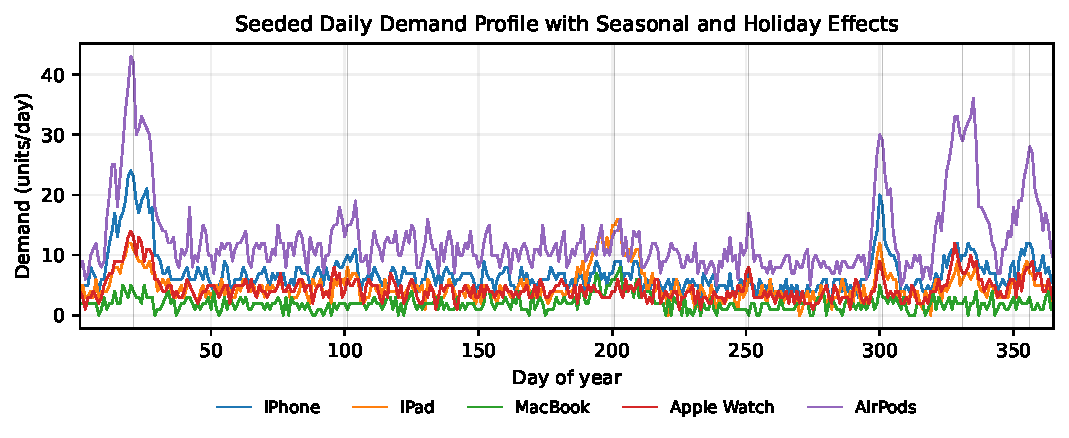
\includegraphics[width=0.92\textwidth]{figures/annual_demand_profile.pdf}
\caption{Illustrative seed-42 daily demand profile generated by the v3 environment for the five product categories. Vertical reference lines indicate configured holiday centers.}\label{fig:demand-profile}
\end{figure*}

\subsection{Ordering Policies}\label{sec:algorithms}

Four ordering policies are trained and evaluated on the environment described above.

\subsubsection{Random Baseline}

Each week, order quantities are drawn independently per product from a continuous uniform distribution over $[0, \mathrm{MAX\_ORDER}_i]$. This baseline has no learning component and serves as a reference point for measuring the value added by the three learned policies.

\subsubsection{Tabular Q-Learning and SARSA}

Following Watkins and Dayan~\cite{bib20}, a per-product Q-table is maintained over a discretized (inventory bucket, forecast bucket) state, with 14 inventory buckets shared across products and 10 product-specific forecast buckets. Each product has its own discrete set of candidate order levels (e.g., iPhone: 0, 5, 10, 15, 20, 30, 40, 50 units), and the agent selects, independently per product, the order level with the highest Q-value under an $\varepsilon$-greedy policy. SARSA~\cite{bib21} uses the identical state discretization, action set, and hyperparameters, but is on-policy: its temporal-difference target uses the value of the action actually taken next under the same $\varepsilon$-greedy policy rather than the maximum over next-state actions, which makes it more conservative in the presence of exploration noise. Both agents use learning rate $0.1$, discount factor $\gamma = 0.99$, and $\varepsilon$ decaying from $0.3$ to a floor of $0.01$ (decay factor $0.995$ per episode) over 200 training episodes.

\begin{algorithm}
\caption{Per-product tabular update (Q-learning / SARSA)}\label{algo:qlearning}
\begin{algorithmic}[1]
\Require learning rate $\alpha=0.1$, discount $\gamma=0.99$, exploration $\varepsilon$
\For{episode $=1$ to $200$}
  \State $s \gets \mathrm{env.reset()}$
  \If{SARSA} $a \gets \varepsilon\text{-greedy}(Q, s)$ \EndIf
  \While{episode not done}
    \If{Q-learning} $a \gets \varepsilon\text{-greedy}(Q, s)$ \EndIf
    \State $s', r, \mathrm{done} \gets \mathrm{env.step}(a)$
    \If{Q-learning}
      \State $\mathrm{target} \gets r/5 + \gamma \max_{a'} Q(s', a')$
    \Else \Comment{SARSA}
      \State $a' \gets \varepsilon\text{-greedy}(Q, s')$
      \State $\mathrm{target} \gets r/5 + \gamma\, Q(s', a')$
    \EndIf
    \State $Q(s,a) \gets Q(s,a) + \alpha\,\big(\mathrm{target} - Q(s,a)\big)$
    \State $s \gets s'$; \ \ (SARSA: $a \gets a'$)
  \EndWhile
  \State $\varepsilon \gets \max(\varepsilon \cdot 0.995,\ 0.01)$
\EndFor
\end{algorithmic}
\end{algorithm}

\subsubsection{SAC-AlphaLR}\label{subsec:sac}

The deep actor-critic agent is denoted SAC-AlphaLR, following the terminology of Zhang, He, and Zheng~\cite{bib1} and the project implementation. The policy follows the Soft Actor-Critic formulation of Haarnoja et al.~\cite{bib3} with automatic temperature tuning~\cite{bib23}. The actor is a feedforward network (state dimension 26, two hidden layers of 256 units, ReLU activations) with separate mean and log-standard-deviation heads (log-std clamped to $[-20, 2]$) over the 5-dimensional action space; actions are sampled via the reparameterization trick, squashed through $\tanh$, and rescaled to $[0, \mathrm{MAX\_ORDER}]$. Two independent critic networks (input dimension $26+5=31$, two hidden layers of 256 units, scalar output) form a twin-Q critic used to mitigate value overestimation. The temperature $\alpha$ is optimized against a target entropy $\mathcal{H}_{\text{target}} = -5$ (the negative of the action dimensionality), via
\begin{equation}
\mathcal{L}(\alpha) = -\,\mathbb{E}\big[\log\alpha \cdot (\log \pi(a|s) + \mathcal{H}_{\text{target}})\big]
\label{eq:alpha}
\end{equation}
All three networks (actor, critic, temperature) use Adam with learning rate $3\times 10^{-4}$; the discount factor is $\gamma=0.99$ and the target-network soft-update coefficient is $\tau = 0.005$. Gradient norms for the actor and critic losses are clipped to $1.0$. According to the supplied v3 training record, the checkpoint was trained for 300 episodes with 2{,}000 initial exploratory interactions before policy-driven updates. At evaluation time the agent acts deterministically ($\tanh$ of the mean, without sampling).

\section{Experimental Setup}\label{sec4}
% [AI-EDITED] New section, written from the actual evaluation protocol used
% in dashboard/backend/rollout.py (matches paper_v1.md Section 5).

All four policies were evaluated over the same 52-week horizon of \texttt{WeeklyRetailEnv} using the v3 demand and business configuration described in Section~\ref{subsec:demand}. Q-learning and SARSA were trained for 200 episodes before evaluation; the supplied v3 record reports that SAC-AlphaLR used a checkpoint trained for 300 episodes with 2{,}000 initial exploratory interactions. The random baseline required no training. The reported values correspond to the documented v3 evaluation run. Because only one run is available, the comparison is descriptive and does not include confidence intervals.

\clearpage
\section{Results}\label{sec5}
% [AI-EDITED] New section; all figures below are measured directly from a
% real run of dashboard/backend/rollout.py, not illustrative placeholders.

Table~\ref{tab:results} reports the full-year (52-week) business outcomes for each policy.

\begin{table}[!h]
\centering
\caption{Annual v3 results by policy (VND, billions unless noted)}\label{tab:results}
\begin{tabular}{@{}lcccc@{}}
\toprule
Policy & Total cost & Revenue & Net profit & Stockout units \\
\midrule
Random       & 183.03 & 119.69 & $-63.34$ & 4{,}973 \\
Q-learning   & 158.35 & 174.41 & $16.06$  & 2{,}365 \\
SARSA        & 161.36 & 170.20 & $8.84$   & 2{,}472 \\
SAC-AlphaLR  & 156.78 & 181.55 & $24.77$  & 2{,}039 \\
\botrule
\end{tabular}
\end{table}

\begin{figure}[!h]
\centering
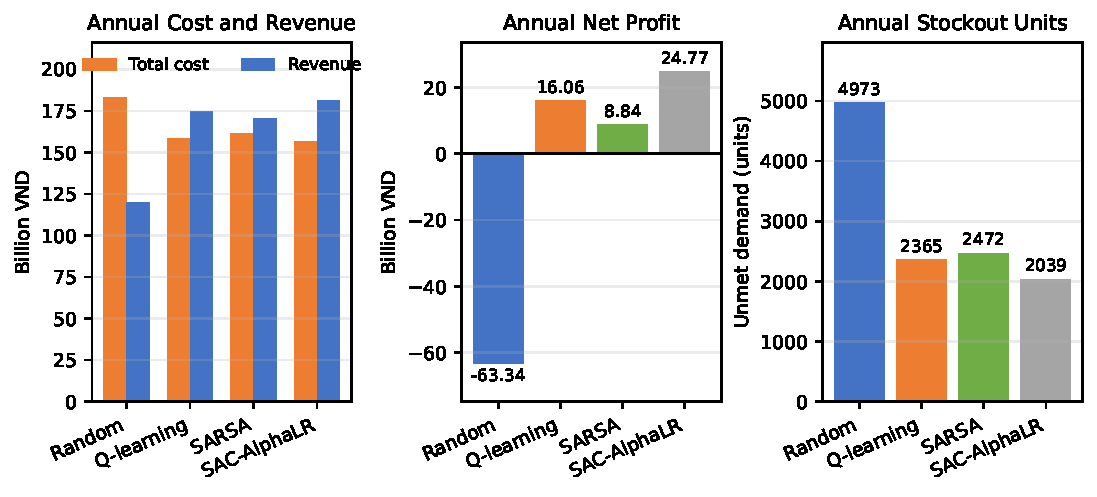
\includegraphics[width=0.92\textwidth]{figures/policy_performance.pdf}
\caption{Annual v3 cost, revenue, net profit, and stockout units for the four evaluated policies. Values correspond to the documented evaluation run in Table~\ref{tab:results}.}\label{fig:policy-performance}
\end{figure}

SAC-AlphaLR is the strongest policy on every reported v3 outcome: its cost is 156.78 billion VND, revenue is 181.55 billion VND, net profit is 24.77 billion VND, and unmet demand is 2{,}039 units. Relative to the random baseline, this corresponds to a 14.3\% cost reduction and a 59.0\% reduction in stockout units. Q-learning and SARSA also achieve positive profit, at 16.06 and 8.84 billion VND respectively. Q-learning performs better than SARSA in v3 on cost, revenue, profit, and stockouts.

\begin{figure}[!h]
\centering
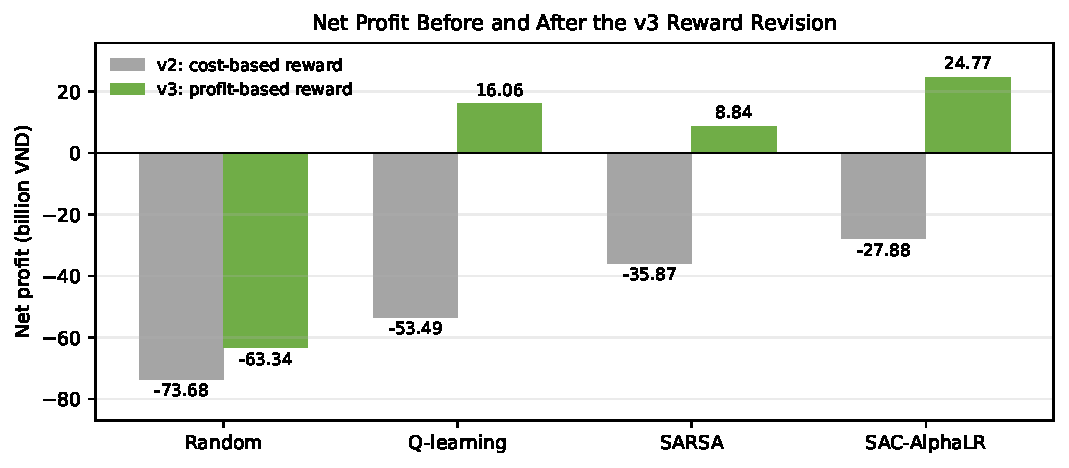
\includegraphics[width=0.86\textwidth]{figures/version_profit_comparison.pdf}
\caption{Net profit reported for the v2 and v3 system versions. The versions differ in reward definition, retail markup, SAC training duration, exploration warm-up, and evaluation realization; the figure is therefore a system-level comparison rather than a controlled reward ablation.}\label{fig:version-profit}
\end{figure}

Figure~\ref{fig:version-profit} shows that the three learned policies move from negative profit in v2 to positive profit in v3, while the random baseline remains negative. This change is consistent with correcting the reward to credit sales revenue and increasing the common retail markup from 25\% to 40\%. However, because several settings changed together, this comparison alone does not isolate the causal contribution of any single revision.

\section{Discussion}\label{sec6}
% [AI-EDITED] New section, adapted from paper_v1.md Section 7.

\textbf{The learned policies are profitable in v3.} Revenue exceeds total cost for Q-learning, SARSA, and SAC-AlphaLR, whereas the random policy loses 63.34 billion VND. The profit-based reward resolves a structural defect in the earlier objective: a cost-only agent was charged for orders but never credited for the sales enabled by those orders, encouraging under-ordering. Under the revised objective and 40\% markup, learned policies are rewarded for purchasing inventory when the expected sales value offsets procurement, storage, and shortage costs.

\textbf{On-policy versus off-policy comparison.} Q-learning outperforms SARSA in v3, earning 16.06 rather than 8.84 billion VND and producing 2{,}365 rather than 2{,}472 stockout units. One plausible explanation is that the off-policy maximum-value target exploits the corrected profit signal more aggressively than SARSA's on-policy update under the shared discretization. This finding should not be over-generalized beyond this evaluation run, since their relative performance is problem-, seed-, and discretization-dependent~\cite{bib22}.

\textbf{Deep actor-critic advantage.} SAC-AlphaLR outperforms both tabular methods, consistent with its access to a continuous action space and a non-discretized state representation. This is consistent with the broader finding of Gijsbrechts et al.~\cite{bib5} that deep RL offers the largest advantage over classical heuristics and simpler RL baselines precisely when the action and state spaces are large or continuous and the constraint structure does not decompose cleanly per product, which is the case for the shared floor-space budget studied here.

\section{Limitations and Future Work}\label{sec7}
% [AI-EDITED] New section, adapted from paper_v1.md Sections 7-8.

The v3 results come from a single documented evaluation run; no confidence intervals or repeated-seed variance estimates are available. A stronger evaluation should average results over multiple training and evaluation seeds. The 40\% markup was selected after the 25\% setting still produced negative profit, so the absolute profit values demonstrate behavior under the revised scenario rather than externally validated commercial profitability. A controlled ablation is also needed to separate the effects of the profit-based reward, markup change, longer SAC training, and longer exploratory warm-up. Further work should add a fixed-temperature SAC baseline, learning curves, and sensitivity analysis for margin, shortage penalty, demand intensity, and floor capacity. Finally, the environment assumes zero lead time and a single retail echelon; adding lead time and an upstream warehouse would enable closer comparison with the multi-echelon studies in Section~\ref{sec2}.

\section{Conclusion}\label{sec8}
% [AI-EDITED] New section, adapted from paper_v1.md Section 8.

This paper presented a weekly, floor-space-constrained retail inventory MDP for a five-category Apple store and compared random ordering, Q-learning, SARSA, and SAC-AlphaLR. Version 3 corrects the reward to maximize scaled net profit and uses a common 40\% retail markup. In the documented 52-week evaluation, SAC-AlphaLR is the best performer, with cost of 156.78 billion VND, revenue of 181.55 billion VND, profit of 24.77 billion VND, and 2{,}039 stockout units. Q-learning and SARSA also earn positive profit, while the random policy remains unprofitable. These findings show that revenue must be represented in the replenishment objective, but they remain conditional on one evaluation run and a calibrated margin assumption. Multi-seed evaluation, controlled ablations, learning curves, and business-parameter sensitivity are required before broader conclusions can be drawn.

\backmatter

\bmhead{Supplementary information}

Not applicable.

\bmhead{Acknowledgements}

Not applicable.
% [AI-EDITED] Both backmatter items above were placeholder template text;
% replaced with "Not applicable" pending author input. Please fill in if
% there is a funding body or supplementary file to disclose.

\section*{Declarations}
% [AI-EDITED] Filled in with best-guess defaults for a simulation-only study
% with no human/animal subjects. Please review every line before submission,
% especially Data availability and Code availability.

\begin{itemize}
\item \textbf{Funding:} Not applicable.
\item \textbf{Conflict of interest/Competing interests:} The authors declare no competing interests.
\item \textbf{Ethics approval and consent to participate:} Not applicable. This study is a computational simulation and does not involve human participants, human data, or animal subjects.
\item \textbf{Consent for publication:} Not applicable.
\item \textbf{Data availability:} Not applicable. This study does not use any external dataset; all demand data are synthetically generated at runtime by the holiday-aware demand generator described in Section~\ref{subsec:demand}, whose parameters are fully specified in Table~\ref{tab:holiday} and can be regenerated exactly from the equations and parameters reported in this paper.
\item \textbf{Materials availability:} Not applicable.
\item \textbf{Code availability:} The environment, agent implementations, training pipeline, and evaluation interface are available at \url{https://github.com/HaoTrieuQuoc/Reinforcement-Learning-with-Inventory-Inbounding}.
\item \textbf{Author contribution:} [Author: please fill in individual author contributions, e.g., using CRediT taxonomy roles.]
\end{itemize}

\bibliography{sn-bibliography}
% common bib file

\end{document}
